\subsection*{Structure d'une partie}

% Label pour le référencement
\label{game}

\subsection*{Problématique}

Le nerf du projet se trouve dans l'implémentation d'une partie. Elle doit permettre de jouer chaque tour séparément, connaître l'état du tour précédent et ainsi pouvoir avoir un historique de la partie. Ce qui sera notamment très utile lors de la création de l'interface mais aussi pour pouvoir jouer de manière indépendante plusieurs parties. (cf \ref{evaluator} et \ref{cli})
\subsection*{Architecture}

\subsubsection*{Structure de tour}

\begin{lstlisting}[frame=single, caption={Implémentation de la structure turn\_t}]
struct turn_t
{
	struct market_t market;
	struct guild_t guild;
	struct player_t players[MAX_PLAYERS];
	unsigned int current_player;
	unsigned int points_to_win;
	unsigned int display; /* Used to display in other functions*/
	unsigned int num_player;
	unsigned int id;
	struct game_parameters params;
	struct context context;
};
\end{lstlisting}

Chaque tour possède la copie de la partie à un instant t.\\
On y retrouve l'état du marché, de la guilde et les inventaires des joueurs à l'issue du tour. Mais également le contexte de ce qu'il s'est passé dans le tour (cf \ref{cli}).

Chaque tour possède volontairement beaucoup d'informations sur la partie car cela va permettre de jouer énormément avec ces paramètres lorsque l'utilise en paramètre de fonction (pour les faveurs et les pouvoirs notamment, cf \ref{skills}).

\subsubsection*{Structure de partie}

\begin{lstlisting}[frame=single, caption={Implémentation de la structure game\_t}]
struct game_t
{
    // +1 for the init state, +1 for the final state
    struct turn_t turns[MAX_MAX_TURNS + 1 + 1]; 
    unsigned int num_turns;
    unsigned int current_turn_index;
};
\end{lstlisting}

Chaque partie stocke l'ensemble des tours qui ont été joués, et contient au plus\\ MAX\_MAX\_TURNS tours (toujours pour éviter l'utilisation de \code{malloc} cf \ref{nomalloc}).\\
num\_turns indique le nombre de tours maximum de la partie (par défaut 10 mais peut être spécifié avec le paramètre -m) et current\_turn\_index l'indice du tour actuellement joué.

\subsection*{Fonctionnement d'une partie}

\subsubsection*{Initialisation de la partie}
Pour initialiser une nouvelle partie, on utilise la fonction \code{init\_game} avec les paramètres souhaités.
\lstset{language=C, style=code}
\begin{lstlisting}[frame=single]
/*
	Init game with params
*/
void init_game(struct game_t*, struct game_parameters);
\end{lstlisting}

\begin{lstlisting}[frame=single, caption={Structure des paramètres de la partie}]
struct game_parameters
{
	unsigned int max_turns;
	unsigned int points_to_win;
	unsigned int builder_seed;
	unsigned int market_seed;
	unsigned int random_seed;
	unsigned int display;
	unsigned int num_player;
};
\end{lstlisting}

La fonction \code{init\_game} modifie le premier tour de la partie en initialisant toutes les instances et en imposant les paramètres de la partie.\\
Le tour est alors sauvegardé (cf \ref{save}) et on peut lancer la partie avec \code{play\_game}.

\subsubsection*{Particularité de \code{rand}}
La fonction \code{rand} étant non ré-entrante, il s'agit de l'unique endroit où \code{srand} est appelée. \code{srand} est appelée une fois lors de l'initialisation des architectes (cf \ref{builders}) et une fois lors de l'initialisation des jetons (cf \ref{tokens}) afin de permettre la création de decks aléatoires indépendants. \\
\code{srand} est alors appelée une dernière fois avec \code{random\_seed} pour initialiser le hasard du reste des actions prises dans la partie.

\begin{figure}[H]
    \centering
    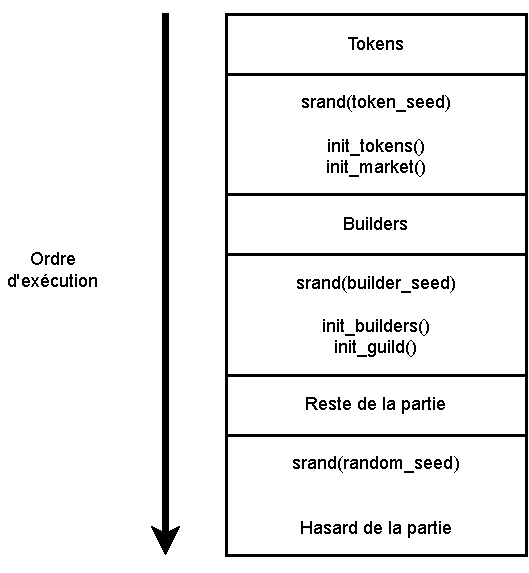
\includegraphics{img/utilisation_srand.pdf}
    \caption{Utilisation de \code{srand}}
    \label{fig:sranduse}
\end{figure}

\subsubsection*{Exécution d'un tour}

\begin{lstlisting}[frame=single, caption={Implémentation de l'exécution d'un tour}]
struct turn_statistics turn_play(struct turn_t* current_turn)
{
    /* Favors execution */
    
	/*
        Take a random decision and check if it's possible to hire a builder
	*/
	unsigned int random_choice = rand() % 100; 
	struct builder_t* builder_to_buy = select_affordable_builder(guild, current_player);

	if ((random_choice < 50) && (builder_to_buy != NULL)) 
	{
		  /* Hire builder and execute associated skills */ 
	}
	else if (random_choice < 90)
	{
		/* Pick tokens and execute associated skills  */
	}
	else 
	{
		/* Skip turn */
	}

}
\end{lstlisting}

A l'aide de la fonction \code{turn\_play}, le tour qui est passé en paramètre est joué.

On s'occupe dans un premier temps des faveurs (cf \ref{favors}) puis on joue le reste du tour. Pour cela on récupère le premier architecte achetable (cf \ref{canbuy}) et on décide d'une action.

\noindent Le joueur a :
\begin{itemize}
    \item 50$\%$ de chance de recruter un architecte (s'il n'en a pas la possibilité, il pioche des jetons)
    \item 40$\%$ de chance de piocher des jetons
    \item 10$\%$ de chance de passer son tour
\end{itemize}

Lorsque le joueur pioche des jetons ou recrute un architecte, on exécute ensuite les pouvoirs éventuellement associés à ce ou ces derniers à l'aide de \code{skill\_exec} (cf \ref{skills}).

On finit par ajouter les actions aux statistiques et au contexte du tour (cf \ref{evaluator} et \ref{cli}).


\subsubsection*{Sauvegarde d'un tour}


\begin{lstlisting}[frame=single, caption={Sauvegarde d'un tour}, label=save]

void game_save_turn(struct game_t* game)
{
    /*  things before */
	memcpy(game_get_turn(game, current_turn_index + 1), game_get_current_turn(game), sizeof(struct turn_t));	
    /* change other params */
}
\end{lstlisting}

Lorsque qu'un tour est joué (à l'aide de \code{play\_turn}) on copie l'état actuel de la partie dans la prochaine case du tableau \code{turns} de la structure \code{game}. Ainsi le tour à la case $i$ du tableau correspond à l'état de la partie à l'issue du $i$-eme tour. \\
On en profite pour modifier les paramètres du prochain tour qui doivent l'être.

\subsubsection*{Boucle de jeu}

\begin{lstlisting}[frame=single, caption={Implémentation de la boucle de jeu}]
struct game_statistics game_play(struct game_t* game)
{
    /*
        Game loop
    */
    while (!has_won(current_turn) && current_turn_index <= num_turns)
    {
        struct turn_statistics turn_stats = turn_play(current_turn);
    
        /* Switch to the next turn */
        game_save_turn(game);
        next_player(game_get_current_turn(game));
    }
}
\end{lstlisting}

La boucle de jeu consiste à jouer des tours tant que la partie n'a pas été gagné et que l'on n'ai pas atteint le nombre maximum de tours. On passe au tour suivant en sauvegardant l'état actuel et en changeant de joueur.